% !TEX root = ../../../main.tex
% 来源：中学数学实验教材·第三册（高中数学）
% 章节：函数及其图象 / 一次函数（线性函数）
% 原始文件：4.tex，行 1266-1295
% 类型：tikz
% ---
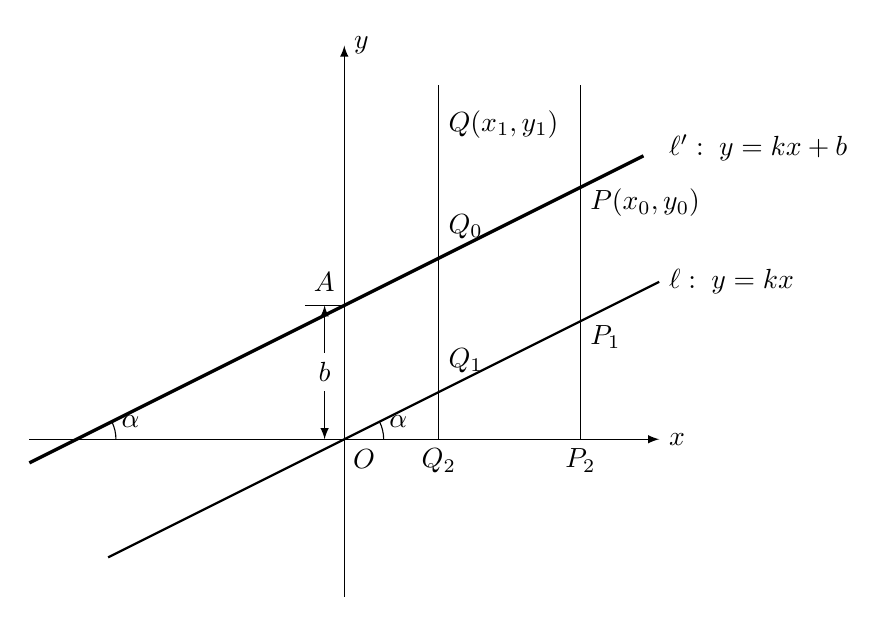
\begin{tikzpicture}[>=latex]
\draw[->] (-4,0)--(4,0)node[right]{$x$};
\draw[->] (0,-2)--(0,5)node[right]{$y$};
\node at (.25,-.25){$O$};

\draw [domain =-3:4, samples=10, thick]plot(\x,{.5*\x});
\draw [domain =-4:3.8, samples=10, very thick]plot(\x,{.5*\x+1.7});
\foreach \x/\xtext in {1.2/Q_2,3/P_2}
{
    \draw (\x,0)node[below]{$\xtext$}--(\x, 4.5);
}

\draw (-.5,1.7)--(0,1.7);
\draw[<->](-.25,1.7)--node[fill=white]{$b$} (-.25,0);
\node at (0,2)[left]{$A$};
\node at (1.2,1)[right]{$Q_1$};
\node at (1.2,2.7)[right]{$Q_0$};
\node at (3,1.3)[right]{$P_1$};
\node at (3,3)[right]{$P(x_0,y_0)$};

\node at (4,2)[right]{$\ell:\; y=kx$};
\node at (4,3.7)[right]{$\ell':\; y=kx+b$};

\draw (.5,0) arc (0:26.56:.5)node[right]{$\alpha$};
\draw (-3.4+.5,0) arc (0:26.56:.5)node[right]{$\alpha$};

\node at (1.2,4)[right]{$Q(x_1,y_1)$};


\end{tikzpicture}
